\documentclass[pdf]{beamer}
\mode<presentation>{} 

\usepackage{hyperref}
\usepackage{pgf}
\usepackage{tikz}
\usetikzlibrary{trees}
\usetikzlibrary{arrows,automata}
\usetikzlibrary{automata,positioning}
\usetikzlibrary{shapes}
\usepackage{tikz-qtree,tikz-qtree-compat}
\usepackage{mathtools,enumerate,amssymb}
\usepackage[utf8]{inputenc}
\usepackage[T1]{fontenc}
\usepackage{graphicx}
\usepackage{multirow}
\usepackage[export]{adjustbox}
\usepackage{wrapfig}
\usepackage{multicol}
\usepackage{enumitem}
\usepackage{flafter}

\definecolor{Blue}{RGB}{0,0,100}
\definecolor{myBlue}{RGB}{0,0,100}
\definecolor{background}{RGB}{255,255,255}



\title{High level models of human-computer behaviour}
\subtitle{Human Computer Interaction}
\AtBeginSection[]{}



\setbeamertemplate{sidebar right}{}
\setbeamertemplate{footline}{%
\hfill\usebeamertemplate***{navigation symbols}
\hspace{1cm}\insertframenumber{}/\inserttotalframenumber}

\graphicspath{{./img/}}



\begin{document}

{\setbeamercolor{background canvas}{bg=background}
\begin{frame}
\vspace{10mm}
\huge{\raggedleft{\color{black}{\textbf{High level models of human-computer behaviour}}}}

\large{\raggedleft{\color{black} Human Computer Interaction}}

\begin{flushright}
\end{flushright}

\fontsize{7pt}{1pt}\selectfont{
Based on slide deck 

\textbf{Part 2: Understanding users and their tasks. High level models of human-computer behaviour}

Human Computer Interaction I: Principles and Design

by

\textbf{Saul Greenberg}
\newline
Professor
\newline
\textbf{University of Calgary, Canada}

\textit{The new slides are marked with a *}
}


\fontsize{5pt}{1pt}\selectfont{ \textcolor{lightgray}
{Slide deck by Saul Greenberg. Permission is granted to use this for non-commercial purposes as long as general credit to Saul Greenberg is clearly maintained.
Warning: some material in this deck is used from other sources without permission. Credit to the original source is given if it is known.}}

\end{frame}}



% Inaintea codului fiecarui slide se vor scrie urmatoarele informatii:
% Nume si prenume student
% Numarul slide-ului corespunzator din prezentarea prof. Saul Greenberg
% Numele imaginilor inserate trebuie sa fie numar_slide_nume_imagine.extensie_imagine


% Jurj Gheorghe Danut
% Slide 1
\begin{frame} \begin{center}
\LARGE{High level models of human-computer behaviour}
\end{center}

\begin{itemize}
\item Are there theories that describe how people interact with computers?

\item \textbf{Quantitative low-level models}
\begin{itemize}
\item Fitts's Lae
\item Keystroke level model
\item ...
\end{itemize}

\item \textbf{Qualitative high-level models}
\begin{itemize}
\item Shneiderman’s syntactic/semantic model
\item Norman’s stages of human interaction
\item ...
\end{itemize}
\end{itemize}

\bigskip
\bigskip \bigskip
\end{frame}



% Jurj Gheorghe Danut
% Slide 2
\begin{frame}
\vspace{8mm}
\textcolor{myBlue}{\textbf{\Large{High-level models of human-computer behaviour}}}

\textcolor{red}{\rule{10cm}{1mm}}

\begin{itemize}
\item[\textcolor{black}{•}] {Developing Theories in HCI }
	\begin{itemize}
	\item[\textcolor{black}{--}] must explain and predict human behaviour in the human-computer system
	\newline
	\item[\textcolor{black}{--}] must work in a wide variety of task situations
	\newline
	\item[\textcolor{black}{--}]must work within broad spectrum of system designs and implementations
	\newline
	\end{itemize}
\end{itemize}
\end{frame}



\begin{frame}
\vspace{8mm}
\textcolor{myBlue}{\textbf{\Large{High-level models of human-computer behaviour}}}

\textcolor{red}{\rule{10cm}{1mm}}

\begin{itemize}
\item[\textcolor{black}{•}] \textbf{Low-level theories can be used to predict human performance}
	\begin{itemize}
	\item[\textcolor{black}{--}] Fitts’s law
		\begin{itemize}
        \begin{scriptsize}
		\item[\textcolor{black}{•}] time to select an item with a pointing device
        \end{scriptsize}
		\end{itemize}
	\item[\textcolor{black}{--}] Keystroke level model 
		\begin{itemize}
        \begin{scriptsize}
		\item[\textcolor{black}{•}] sums up times for keystroking, pointing, homing, drawing, thinking and waiting
        \end{scriptsize}
        \end{itemize}
\end{itemize}
\end{itemize}
\end{frame}



\begin{frame}
\vspace{8mm}
\textcolor{myBlue}{\textbf{\Large{*Fitts's Law}}}

\textcolor{red}{\rule{10cm}{1mm}}

  \begin{itemize}
  	\item[\textcolor{black}{•}] The \textbf{time required to rapidly move to a target area is a function of the ratio between the distance to the target and the width of the target}
  	\newline
  	
  	\item[\textcolor{black}{•}] used to model the act of \textit{pointing} (physically or virtually)
  	\newline
  	
  	\item[\textcolor{black}{•}] $MT = a + b \times log_2(2 \times D/W)$
  	\begin{itemize}
  		\item[--] MT - time to hit the target
  		\item[--] a,b - empirically determined constants
  	\end{itemize}
  \end{itemize}

  \begin{figure}
  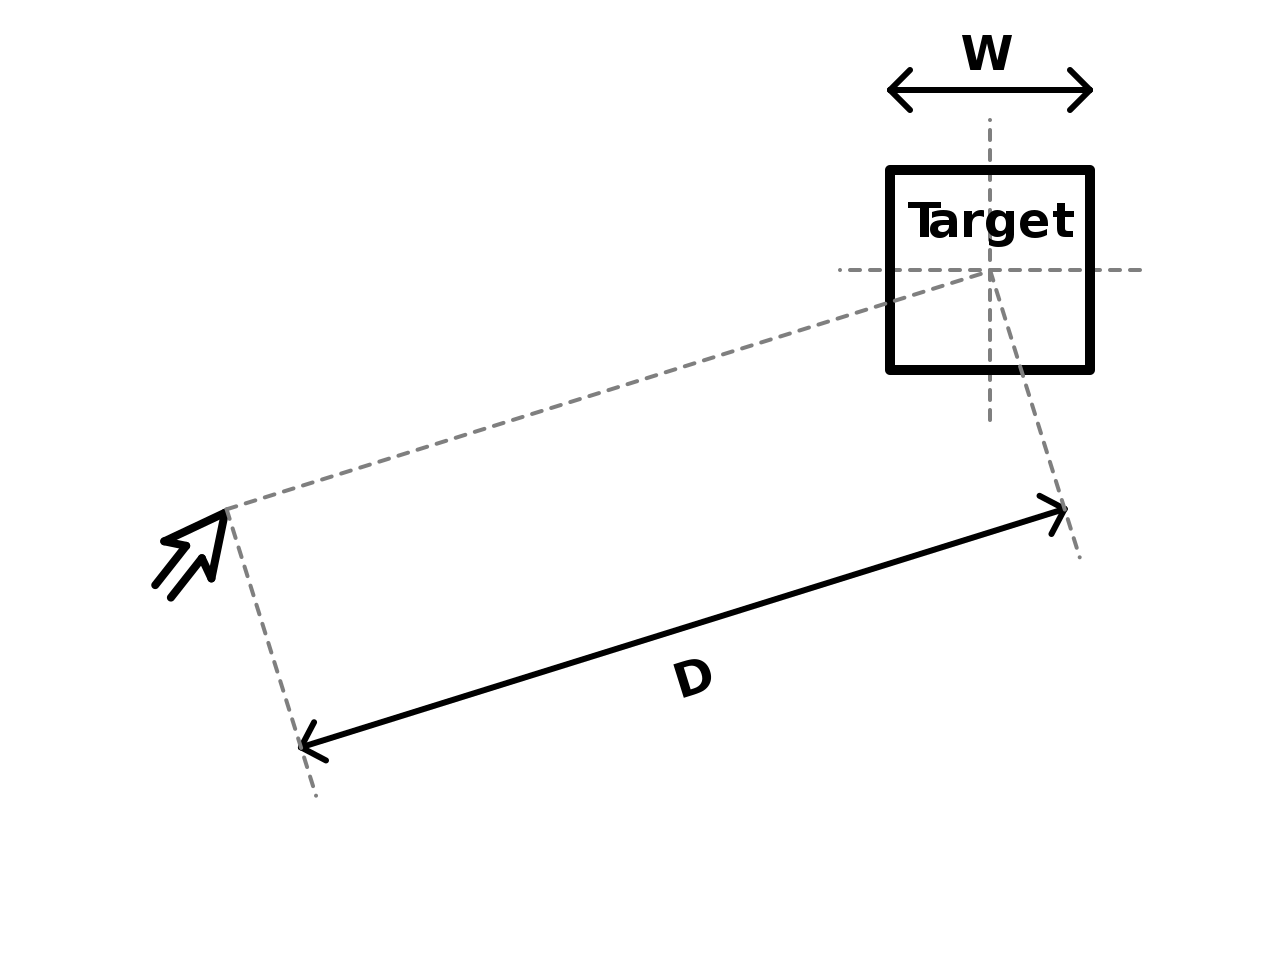
\includegraphics[scale=0.1]{Fitts_Law.png}
  \end{figure}
  
\end{frame}



\begin{frame}
\vspace{8mm}
\textcolor{myBlue}{\textbf{\Large{*Keystroke level modelling}}}

\textcolor{red}{\rule{10cm}{1mm}}

  \begin{itemize}
  	\item[\textcolor{black}{•}] estimates the ideal task time
  	\newline
  	
  	\item[\textcolor{black}{•}] based on a detailed analysis of all elementary steps that users need to go through to reach the goal of the task
  	\newline
  	
  	\item[\textcolor{black}{•}] it works by summarizing all the elementary steps (keystroke, typing, mouse click, homing, pointing, \textbf{mental operations}, system response) which are needed for finalizing the task
  \end{itemize}
  
\end{frame}



\begin{frame}
\vspace{8mm}
\textcolor{myBlue}{\textbf{\Large{*Keystroke level modelling - An example}}}

\textcolor{red}{\rule{10cm}{1mm}}

  \begin{figure}
  \centering
  	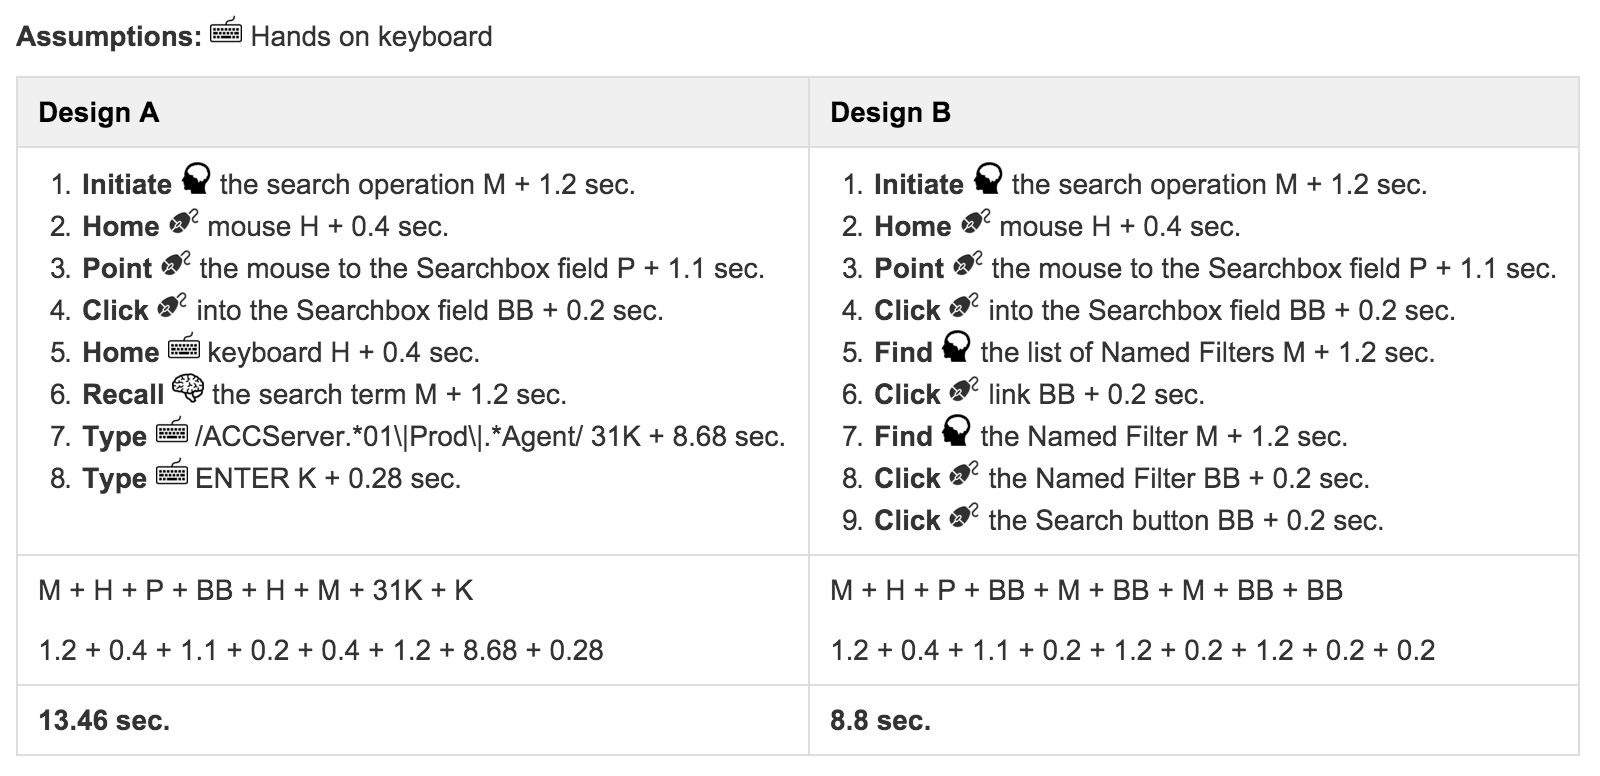
\includegraphics[scale=0.2]{KLM_example.png} 
  \end{figure}
  
  Peter Zalman, \textbf{Key-stroke Level Model}
  
  \url{https://medium.com/enterprise-ux/key-stroke-level-model-213dd054e5c7}
  
\end{frame}



\begin{frame}
\vspace{8mm}
\textcolor{myBlue}{\textbf{\Large{*High-level models of human-computer behaviour}}}

\textcolor{red}{\rule{10cm}{1mm}}

\begin{itemize}
\item[\textcolor{black}{•}] Uses of these low-level theories
	\begin{itemize}
		\item[--] compare two design variants
		\item[--] common benchmarking
		\item[--] measure improvement in case of reduce time-on-task by N\% design goals		
		\item[--] user testing (in case evaluation with real users is not possible)
	\end{itemize}
\end{itemize}
\end{frame}



\begin{frame}
\vspace{8mm}
\textcolor{myBlue}{\textbf{\Large{High-level models of human-computer behaviour}}}

\textcolor{red}{\rule{10cm}{1mm}}

\begin{itemize}
\medskip
\item[\textcolor{black}{•}] \textbf{General models that explain human behaviour with machines/computers}
	\begin{itemize}
    \begin{footnotesize}
	\item[\textcolor{black}{--}] Syntactic/semantic model (Shneiderman)
	\item[\textcolor{black}{--}] Stages of interaction (Norman)
	\item[\textcolor{black}{--}] all of psychology!
    \end{footnotesize}
	\end{itemize}
\end{itemize}
\end{frame}



% Jurj Gheorghe Danut
% Slide 3
% 3_pic.png
\begin{frame}
\vspace{8mm}
\textcolor{myBlue}{\textbf{\Large{Syntactic/semantic model of user knowledge}}}

\textcolor{red}{\rule{10cm}{1mm}}

  \begin{itemize}
  	\item[\textcolor{black}{•}] \Large A high level model of interaction, developed by Ben Shneiderman 
  \end{itemize}
  \begin{figure}
  	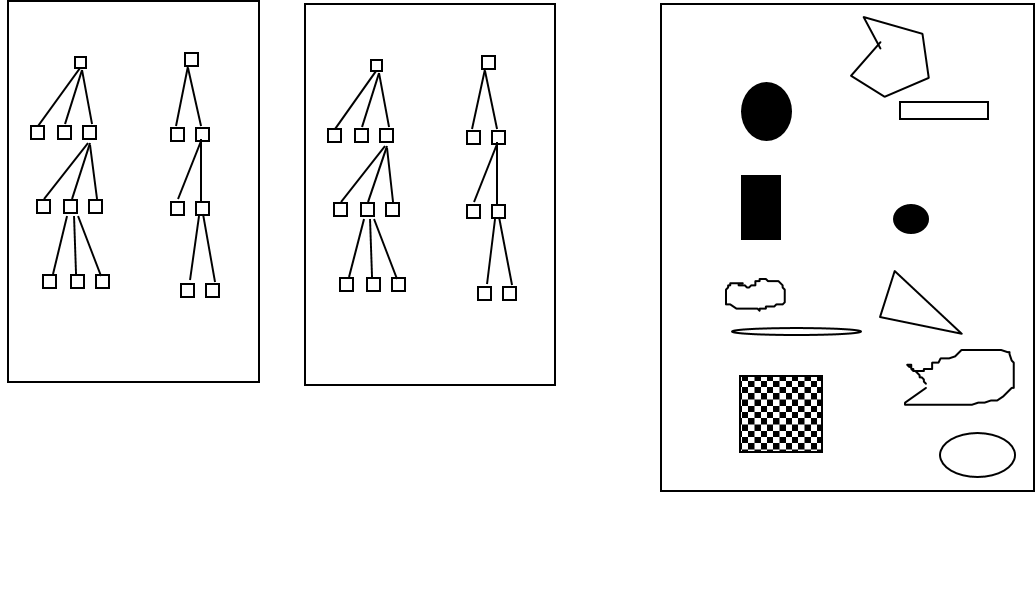
\includegraphics[scale=0.32]{3_pic.png} 
  \end{figure}
  \leavevmode\makebox(0,0){\put(35,170){\selectfont{\footnotesize Action Object}}}
  \leavevmode\makebox(0,0){\put(102,170){\selectfont{\footnotesize Action Object}}}
  \leavevmode\makebox(0,0){\put(45,130){\selectfont{\textbf{Task}}}}
  \leavevmode\makebox(0,0){\put(100,130){\selectfont{\textbf{Computer}}}}
  \leavevmode\makebox(0,0){\put(200,80){\selectfont{\textbf{Syntactic}}}}
  \leavevmode\makebox(0,0){\put(65,80){\selectfont{\textbf{Semantic}}}}
\end{frame}



\begin{frame}
\vspace{8mm}
\textcolor{myBlue}{\textbf{\Large{*Syntactic knowledge}}}

\textcolor{red}{\rule{10cm}{1mm}}

  \begin{figure}
  \centering
  	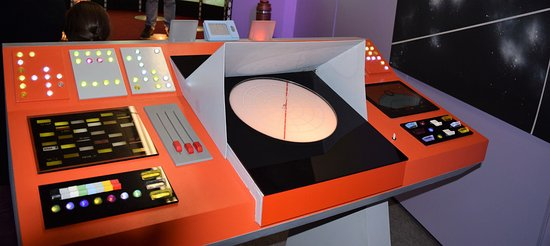
\includegraphics[scale=0.5]{star-trek-map-lovely-transporter-console-at-the-ready-picture-of-star-trek-original.jpg} 
  \end{figure}

Star Trek Transporter console

\url{https://vidasmps.com/star-trek-map/star-trek-map-lovely-transporter-console-at-the-ready-picture-of-star-trek-original/}

\end{frame}



% Jurubita Ilie
% Slide 4
\begin{frame}
\vspace{8mm}
\textcolor{myBlue}{\textbf{\Large{Syntactic knowledge}}}

\textcolor{red}{\rule{10cm}{1mm}}

\begin{itemize}
\begin{small}
\medskip
\item[\textcolor{black}{•}] \textbf{The rules or combinations of commands and signals} \newline
	\begin{itemize}
	\item[\textcolor{black}{--}] seen as device-dependent details of how to use system \newline
	\item[\textcolor{black}{--}] examples: \newline
		\begin{itemize}
        \begin{scriptsize}
		\item[\textcolor{black}{•}] backspace key -	deletes previous character \newline
        \item[\textcolor{black}{•}] right mouse button - raises contextual menu \newline
        \item[\textcolor{black}{•}] grep <word> <file>	- finds a word in a file character\newline
        \item[\textcolor{black}{•}] tab - moves to next field in a form \newline
        \item[\textcolor{black}{•}] dd - deletes current line in vim text editor 
        \end{scriptsize}
        \end{itemize}
	\end{itemize}
\medskip
\end{small}
\end{itemize}
\end{frame}



%Jurubita Ilie
%Slide 5
%5_imag.png
\begin{frame}
\vspace{8mm}
\textcolor{myBlue}{\textbf{\Large{User problems with syntactic knowledge}}}

\textcolor{red}{\rule{10cm}{1mm}}

\begin{small}

	\begin{itemize}
	\item[\textcolor{black}{--}] syntactic details differ between (and within!) systems
		  \begin{itemize}
		  \item[\textcolor{black}{•}] little/arbitrary consistency 
          \item[\textcolor{black}{•}] e.g. 
                 \begin{itemize}
                 \item[\textcolor{black}{--}] :q - quits vim text editor
                  \item[\textcolor{black}{--}] exit - quits current login user
                  \item[\textcolor{black}{--}] Ctrl + X - quits nano text editor
                  \item[\textcolor{black}{--}] q - quits displaying content with less
                 \end{itemize}
          \end{itemize}
	\end{itemize}

\end{small}
\end{frame}



\begin{frame}
\vspace{8mm}
\textcolor{myBlue}{\textbf{\Large{User problems with syntactic knowledge}}}

\textcolor{red}{\rule{10cm}{1mm}}

\begin{small}

	\begin{itemize}
    \item[\textcolor{black}{--}] hard to learn
          \begin{itemize}
		  \item[\textcolor{black}{•}] acquired by rote memorization
          \item[\textcolor{black}{•}] repeated rehearsals to reach competency
          \item[\textcolor{black}{•}] must be frequently applied for retention over time
          \end{itemize}
    \item[\textcolor{black}{--}] easily forgotten
          \begin{itemize}
	      \item[\textcolor{black}{•}] expert/frequent users ok
          \item[\textcolor{black}{•}] novice/casual users troubled by syntactic irregularities         \end{itemize}
	\end{itemize}
    
\medskip
\end{small}
\end{frame}



%Jurubita Ilie
%Slide 6
%6_imag.png
\begin{frame}
\vspace{8mm}
\textcolor{myBlue}{\textbf{\Large{Semantic knowledge: computer concepts}}}

\textcolor{red}{\rule{10cm}{1mm}}

\begin{small}

\begin{itemize}
\item[\textcolor{black}{•}] \textbf{The meaning behind computer concepts}

\item[\textcolor{black}{•}] \textbf{Usually follows a hierarchical structure}
    \begin{itemize}
    \item[\textcolor{black}{--}] high level concepts decomposed to many  low level concepts
    \item[\textcolor{black}{--}] objects
            \begin{itemize}
            \item[\textcolor{black}{•}] e.g. stored information as  directories and files as name,                      length, creation date, owner,...
            \end{itemize}
    \item[\textcolor{black}{--}] actions
            \begin{itemize}
            \item[\textcolor{black}{•}]e.g. saving a file, creating backups, verify access control, etc.
            \end{itemize}
    \end{itemize}
\end{itemize}
\end{small}
\end{frame}



\begin{frame}
\vspace{8mm}
\textcolor{myBlue}{\textbf{\Large{Semantic knowledge: computer concepts}}}

\textcolor{red}{\rule{10cm}{1mm}}

\begin{small}
\begin{itemize}    
\item[\textcolor{black}{•}] \textbf{How it works}

    \begin{itemize}
    \item[\textcolor{black}{--}] people learn computer concepts by
          \begin{itemize}
          \item[\textcolor{black}{•}] meaningful learning
          \item[\textcolor{black}{•}] demonstrations
          \item[\textcolor{black}{•}] explanations of features
          \item[\textcolor{black}{•}] trial by error
          \item[\textcolor{black}{•}] model of concepts (abstract, concrete,analogical)
          \item[\textcolor{black}{--}] e.g. 
			\begin{itemize}
			\item file hierarchies are like file/folder systems
			\end{itemize}			          

          \end{itemize}
     \end{itemize}
\end{itemize}
\end{small}
\end{frame}



%Jurubita Ilie
%Slide 7
\begin{frame}
\vspace{8mm}
\textcolor{myBlue}{\textbf{\Large{Semantic knowledge: computer concepts}}}

\textcolor{red}{\rule{10cm}{1mm}}

\begin{small}

\begin{itemize}
\item[\textcolor{black}{•}] \textbf{Properties of semantic knowledge (computer concepts)}
     \begin{itemize}
     \item[\textcolor{black}{--}] relatively stable in memory
             \begin{itemize}
             \item[\textcolor{black}{•}] high level concepts
             \item[\textcolor{black}{•}] logical structure
             \item[\textcolor{black}{•}] cognitive model produced\newline
             \end{itemize}
             
      \item[\textcolor{black}{--}] usually transferable across computer systems
             \begin{itemize}
             \item[\textcolor{black}{•}] but not always!\newline
             \end{itemize}
      \end{itemize}
      
\item[\textcolor{black}{•}] \textbf{Problems}
      \begin{itemize}
      \item[\textcolor{black}{--}] many people now using computers are not computer scientists!
      \item[\textcolor{black}{--}] must be trained in "computer literacy"
      \item[\textcolor{black}{--}] people prefer to concentrate on task, not on computer knowledge
      \end{itemize}
\end{itemize}
\medskip
\end{small}
\end{frame}



\begin{frame}
\vspace{8mm}
\textcolor{myBlue}{\textbf{\Large{*Semantic knowledge: task concepts}}}

\textcolor{red}{\rule{10cm}{1mm}}

  \begin{figure}
  \centering
  	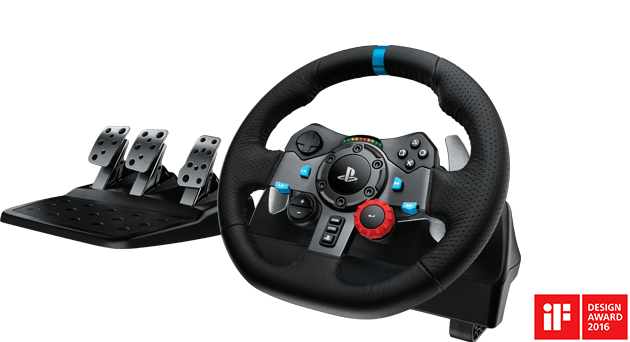
\includegraphics[scale=0.4]{g29-racing-wheel.png} 
  \end{figure}

Racing wheel for Playstation

\url{https://origin-gaming.logitech.com/en-us/product/g29-driving-force}

\end{frame}



\begin{frame}
\vspace{8mm}
\textcolor{myBlue}{\textbf{\Large{Semantic knowledge: task concepts}}}

\textcolor{red}{\rule{10cm}{1mm}}

\begin{small}

\begin{itemize}
\item[\textcolor{black}{•}] \textbf{The meaning behind task concepts}
     \begin{itemize}
     \item[\textcolor{black}{--}] is independent of the computer
     \newline
     \end{itemize}

\item[\textcolor{black}{•}] \textbf{Similar in mechanisms to computer concepts}
             
\item[\textcolor{black}{•}] e.g.      
\begin{itemize}
   \item[\textcolor{black}{--}] how to write a business letter
   	\begin{itemize}
		\item format concerns
   		\item stylistic concerns
   		\item paragraph structure
   		\item etc. 
	\end{itemize}
   \item[\textcolor{black}{--}] creating lecture notes
\end{itemize}
\end{itemize}
\end{small}
\end{frame}



%Jurubita Ilie
%Slide 9
\begin{frame}
\vspace{8mm}
\textcolor{myBlue}{\textbf{\Large{What syntactic/semantic model reveals}}}

\textcolor{red}{\rule{10cm}{1mm}}

\begin{small}

Mapping between three items is extremely important: \textbf{Task semantics to computer semantics to computer syntax}

\begin{itemize}
\item [\textcolor{black}{--}] e.g.
     \begin{itemize}
     \item [\textcolor{black}{•}]task semantics: 	write letter
     \item [\textcolor{black}{•}]computer semantics: 	open a file, use editor, save it to disk
     \item [\textcolor{black}{•}]computer syntax: 	select menu items, key strokes for formatting,...
     \newline
     \end{itemize}
\end{itemize}
\end{small}
\end{frame}



\begin{frame}
\vspace{8mm}
\textcolor{myBlue}{\textbf{\Large{What syntactic/semantic model reveals}}}

\textcolor{red}{\rule{10cm}{1mm}}

\begin{small}

\begin{itemize}
\item [\textcolor{black}{--}]Bad mapping: using latex to write letter
     \begin{itemize}
     \item [\textcolor{black}{•}]aside from task semantics, must also know semantics/syntax of:
            \begin{itemize}
            \item [\textcolor{black}{--}]text editor
            \item [\textcolor{black}{--}]latex
            \item [\textcolor{black}{--}]Unix compiling and printing sequence (to typeset and print)
            \end{itemize}
      \end{itemize}
      
\item [\textcolor{black}{--}]Relatively good mapping: trashcan to throw away files
     \begin{itemize}
     \item [\textcolor{black}{•}]must know mouse syntax of selecting and dragging
     \item [\textcolor{black}{•}]computer semantics almost analogous to task semantics
     \end{itemize}
\end{itemize}
\medskip
\end{small}
\end{frame}



%Jurubita Ilie
%Slide 10
\begin{frame}
\vspace{8mm}
\textcolor{myBlue}{\textbf{\Large{Guidelines suggested by syntactic/semantic model}}}

\textcolor{red}{\rule{10cm}{1mm}}

\begin{small}

\textbf{Reduce the burden of learning a separate computer semantics and syntax, for the task-oriented user}
\newline

\textbf{Methods:}

\begin{itemize}
\item [\textcolor{black}{--}]computer semantics
     \begin{itemize}
     \item [\textcolor{black}{•}]metaphors allow computer artifacts to be represented as task artifacts
           \begin{itemize}
           \item [\textcolor{black}{--}]e.g. office workers: files/folders represent hierarchical directory/file systems
           \end{itemize}
     \item [\textcolor{black}{•}]information hiding
           \begin{itemize}
           \item [\textcolor{black}{--}]don’t force people to know computer concepts that are not   relevant to their work
           \end{itemize}
      \end{itemize}
\end{itemize}
\medskip
\end{small}
\end{frame}



\begin{frame}
\vspace{8mm}
\textcolor{myBlue}{\textbf{\Large{Guidelines suggested by syntactic/semantic model}}}

\textcolor{red}{\rule{10cm}{1mm}}

\begin{small}

\begin{itemize}
\item [\textcolor{black}{--}]computer syntax
      \begin{itemize}
      \item [\textcolor{black}{•}]a little learning should go a long way ...
      \item [\textcolor{black}{•}] should be as understandable as possible (tied to semantics) 
            \begin{itemize}
            \item [\textcolor{black}{--}] e.g. meaningful command names, icons, keyboard shortcuts
            \end{itemize}
      \item [\textcolor{black}{•}] should be as simple as possible and uniformly applicable
            \begin{itemize}
            \item [\textcolor{black}{--}] e.g., object selection with mouse: single click selects, double click activates
            \end{itemize}
      \item [\textcolor{black}{•}] generic commands
            \begin{itemize}
            \item [\textcolor{black}{--}] same command can be applied across different objects
            \end{itemize}
      \item [\textcolor{black}{•}] syntax should be consistent between systems!
      \end{itemize}
\end{itemize}
\medskip
\end{small}
\end{frame}



%Jurubita Ilie
%Slide 11
\begin{frame}
\vspace{8mm}
\textcolor{myBlue}{\textbf{\Large{The Four Stages of an Interaction}}}

\textcolor{red}{\rule{10cm}{1mm}}

\begin{small}

\textbf{Intention, Selection, Execution, Evaluation} (a simplified version of Norman’s 7 stages)

\begin{itemize}
\item [\textcolor{black}{•}]1. \textbf{Forming an intention}
      \begin{itemize}
      \item [\textcolor{black}{--}] "What we want to happen"
      \item [\textcolor{black}{--}]internal mental characterization of a goal
      \item [\textcolor{black}{--}]may comprise goals and sub-goals (but rarely are they well planned)
      \item [\textcolor{black}{--}]similar to task semantics
            \begin{itemize}
            \item [\textcolor{black}{•}]e.g. "begin a letter to Aunt Harriet"
            \end{itemize}
      \end{itemize}
      
\item [\textcolor{black}{•}]2. \textbf{Selecting an action}
      \begin{itemize}
      \item [\textcolor{black}{--}]review possible actions and select most appropriate
      \item [\textcolor{black}{--}]similar to mapping between task and compute semantics
            \begin{itemize}
            \item [\textcolor{black}{•}]e.g. "use the gedit editor to create a file harriet.letter"
            \end{itemize}
       \end{itemize}
\end{itemize}

\end{small}
\end{frame}



% Medvei Mirabela Melinda
% Slide 13
\begin{frame} 
\vspace{8mm}
\textcolor{myBlue}{\textbf{\Large{The Four Stages of an Interaction}}}

\textcolor{red}{\rule{10cm}{1mm}}

\begin{itemize}
	\item[\textcolor{black}{•}] 3. \textbf{Executing the action}
    \smallskip
	\begin{itemize}
    	\item[\textcolor{black}{--}] carry out the action using the computer
        \smallskip
        \item[\textcolor{black}{--}] similar to mapping between semantics and computer syntax
         \smallskip
         \begin{itemize} \begin{scriptsize}
         	\item[\textcolor{black}{•}] e.g. type "gedit harriet.letter"
          \end{scriptsize} \end{itemize}
	\end{itemize}
	\medskip
    
	\item[\textcolor{black}{•}] 4. \textbf{Evaluate the outcome}
    \smallskip
	\begin{itemize}
		\item[\textcolor{black}{--}] check the results of executing the action and compare it with the expectations
        \smallskip
        \begin{itemize}
        \begin{scriptsize}
        	\item[\textcolor{black}{•}] e.g. see if gedit editor is on the display and verify that file name is "harriet.letter"
            \item[\textcolor{black}{•}] requires perception, interpretation, and incremental evaluation
        \end{scriptsize}
        \end{itemize}
	\end{itemize}  
\end{itemize}
\bigskip \bigskip
\end{frame}



% Medvei Mirabela Melinda
% Slide 12
% 12_Picture1.png
\begin{frame}
\vspace{8mm}
\textcolor{myBlue}{\textbf{\Large{The stages of user activities when performing a task}}}

\textcolor{red}{\rule{10cm}{1mm}}

\begin{figure} 
 	\centering
  	\hspace{10px} 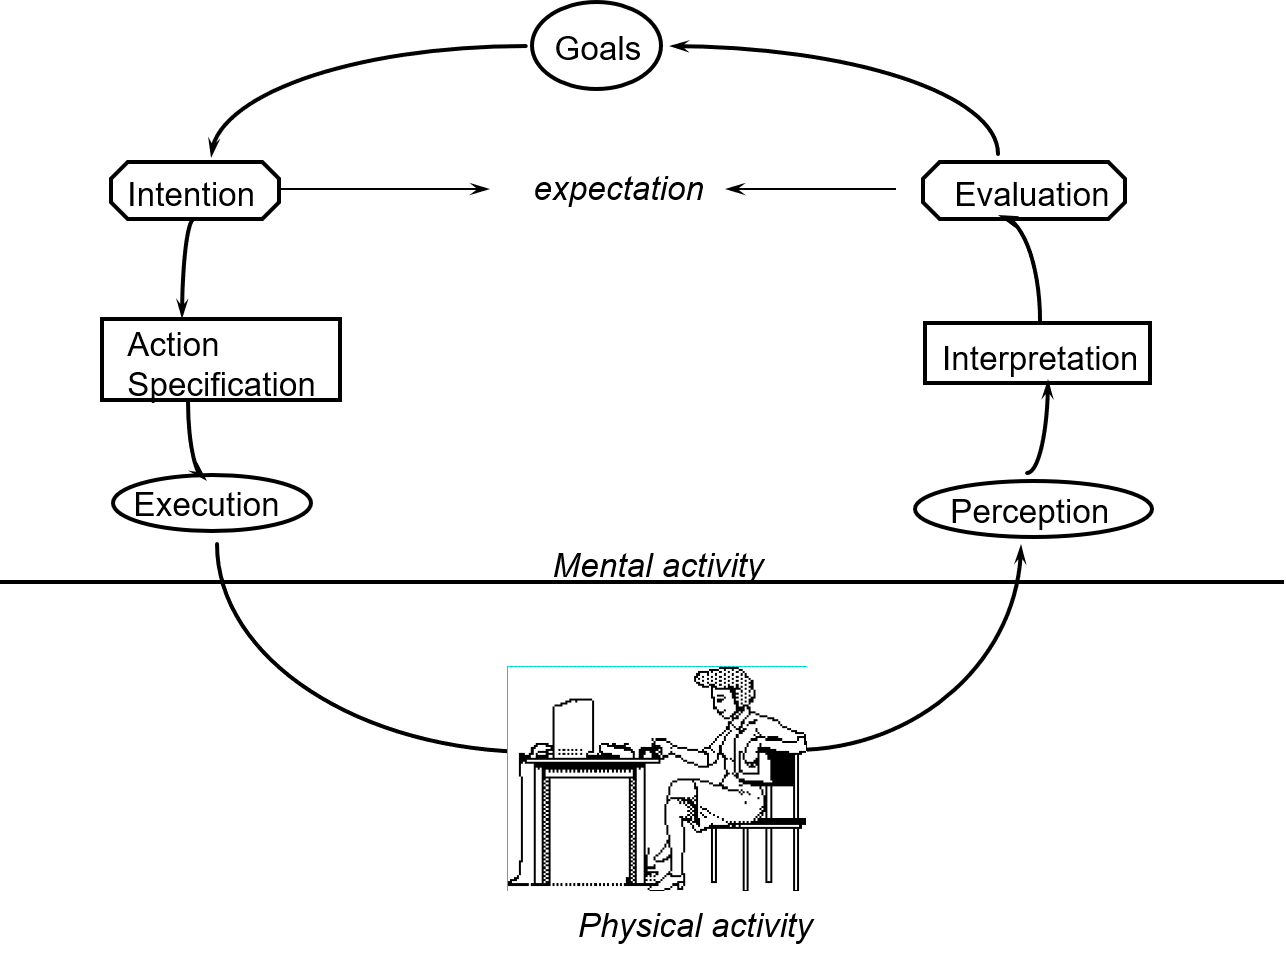
\includegraphics[width=0.85\textwidth]{12_Picture1.png}
\end{figure}
\end{frame}



% Medvei Mirabela Melinda
% Slide 14
% 14_Picture1.png
\begin{frame} 
\vspace{8mm}
\textcolor{myBlue}{\textbf{\Large{A typical task: making a business letter look better}}}

\textcolor{red}{\rule{10cm}{1mm}}

\begin{figure} 
	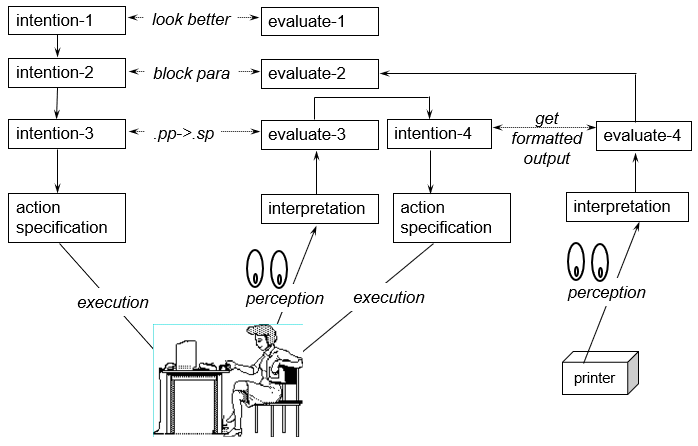
\includegraphics[scale=0.5]{14_Picture1.png}
\end{figure}
\end{frame}



% Medvei Mirabela Melinda
% Slide 15
% 15_Picture1.png
\begin{frame} 
\vspace{8mm}
\textcolor{myBlue}{\textbf{\Large{What the four stages model reveals}}}

\textcolor{red}{\rule{10cm}{1mm}}

\textbf{The "Gulf of Execution"}

\begin{itemize}
        \item[\textcolor{black}{--}] Gulf: amount of effort exerted to transform intentions into selected and executed actions
        
    	\item[\textcolor{black}{--}] do actions provided by system correspond to the intentions of the user?
    	        
        \item[\textcolor{black}{--}] a good system:
        \begin{itemize}
        \begin{scriptsize}
        	\itemsep0.1em
        	\item[\textcolor{black}{\tiny$\bullet$}] direct mappings between intention and selections
        	
            \item[\textcolor{black}{\tiny$\bullet$}]e.g. printing a letter:
            \vspace*{0.01cm}
            \begin{itemize}
            	\itemsep0.1em
            	\item[\textcolor{black}{--}] put document on printer icon
                \item[\textcolor{black}{--}] vs select print from menu
                \item[\textcolor{black}{--}] vs "latex letter.tex; lpr -Palw3 latex.dvi"
                \item[\textcolor{black}{--}] drawing a line: move mouse on graphical display vs "draw (x1, y1, x2, y2)"
            \end{itemize}
        \end{scriptsize}
    \end{itemize}
  \end{itemize}
\end{frame}



\begin{frame} 
\vspace{8mm}
\textcolor{myBlue}{\textbf{\Large{What the four stages model reveals}}}

\textcolor{red}{\rule{10cm}{1mm}}

\textbf{The "Gulf of Execution"}

\begin{figure} 
	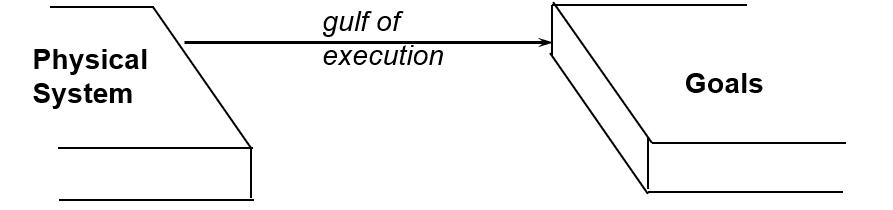
\includegraphics[scale=0.5]{15_Picture1.png}
\end{figure}
\end{frame}



% Medvei Mirabela Melinda
% Slide 16
% 16_Picture1.png
\begin{frame} 
\vspace{8mm}
\textcolor{myBlue}{\textbf{\Large{What the four stages model reveals}}}

\textcolor{red}{\rule{10cm}{1mm}}

\textbf{The "Gulf of Evaluation"}

	\begin{itemize} 
    \begin{small}
    	\itemsep0.25em
        \item[\textcolor{black}{--}] Gulf: amount of effort exerted to interpret feedback
    	        
    	\item[\textcolor{black}{--}] can feedback be interpreted in terms of intentions and expectations?

        \item[\textcolor{black}{--}] a good system: 
		\begin{itemize}        
        	\item feedback easily interpreted as task expectations
        \vspace*{0.1cm}
        \begin{itemize}
        	\item[\textcolor{black}{\tiny$\bullet$}] \scriptsize{ e.g. graphical simulation of text page being printed}
        \end{itemize}
        \end{itemize}
         \item[\textcolor{black}{--}] a bad system: 
		 \begin{itemize}		          
         	\item no feedback or difficult to interpret feedback
         \vspace*{0.1cm}
         \begin{itemize}
        	\item[\textcolor{black}{\tiny$\bullet$}] \scriptsize{ e.g. Unix: "\$", "bus error", "command not found"}
        \end{itemize}
        \end{itemize}
  	\end{small}
  	\end{itemize}
\end{frame}



\begin{frame} 
\vspace{8mm}
\textcolor{myBlue}{\textbf{\Large{What the four stages model reveals}}}

\textcolor{red}{\rule{10cm}{1mm}}

\textbf{The "Gulf of Evaluation"}

\begin{figure} 
	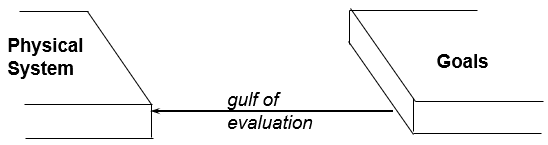
\includegraphics[scale=0.7]{16_Picture1.png}
\end{figure}
\end{frame}



% Medvei Mirabela Melinda
% Slide 17
% 17_Picture1.png

\begin{frame}
\vspace{8mm}
\textcolor{myBlue}{\textbf{\Large{Bridging the Gulf of Execution and Evaluation}}}

\textcolor{red}{\rule{10cm}{1mm}}

\begin{figure} 
\centering
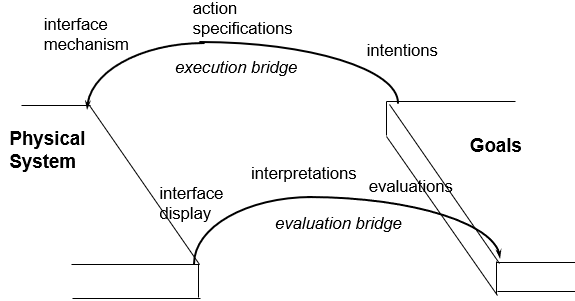
\includegraphics[scale=0.72]{17_Picture1.png}
\end{figure}
\end{frame}



% Medvei Mirabela Melinda
% Slide 18
\begin{frame} 
\vspace{8mm}
\textcolor{myBlue}{\textbf{\Large{Using four stages to ask design questions}}}

\textcolor{red}{\rule{10cm}{1mm}}

\textbf{How easily can a user:}

	\begin{itemize} 
    	\itemsep0.35em
    	\item[\textcolor{black}{--}] determine the function of the system?
        \item[\textcolor{black}{--}] tell what actions are possible?
        \item[\textcolor{black}{--}] determine mapping from intention to selection?
        \item[\textcolor{black}{--}] perform the action?
        \item[\textcolor{black}{--}] tell what state the system is in?
        \item[\textcolor{black}{--}] determining mapping from system state to interpretation?
        \item[\textcolor{black}{--}] tell if system is in the desired state?
  	\end{itemize}
\end{frame}



% Medvei Mirabela Melinda
% Slide 19
\begin{frame} 
\vspace{8mm}
\textcolor{myBlue}{\textbf{\Large{Using four stages to ask design questions}}}

\textcolor{red}{\rule{10cm}{1mm}}

\textbf{Questions similar to principles of good design:}

	\begin{itemize} 
    	\item[\textcolor{black}{--}] visibility
        \begin{itemize}
        	\item[\textcolor{black}{\tiny$\bullet$}] \small{ can see state of application and alternatives for actions}
        \end{itemize}
        
        \item[\textcolor{black}{--}] good conceptual model
        \begin{itemize}
        	\item[\textcolor{black}{\tiny$\bullet$}] \small{consistency in presentations of operations and results}
            \item[\textcolor{black}{\tiny$\bullet$}] \small{coherent system image}
        \end{itemize}
        
        \item[\textcolor{black}{--}] good mappings
        \begin{itemize}
        	\item[\textcolor{black}{\tiny$\bullet$}] \small{ relations between}
            \begin{itemize} \begin{scriptsize}
            	\itemsep0.15em
            	\item[\textcolor{black}{--}] actions and results
                \item[\textcolor{black}{--}] controls and their effects
                \item[\textcolor{black}{--}] system state and what is visible
            \end{scriptsize} \end{itemize}
        \end{itemize}
        
        \item[\textcolor{black}{--}] feedback
        \begin{itemize}
        	\item[\textcolor{black}{\tiny$\bullet$}] \small{ full and continuous feedback about results of actions}
		\end{itemize}
  	\end{itemize}
\end{frame}



\begin{frame} 
\vspace{8mm}
\textcolor{myBlue}{\textbf{\Large{Using four stages to ask design questions}}}

\textcolor{red}{\rule{10cm}{1mm}}

\textbf{Questions similar to principles of good design:}

\begin{itemize}
    \item[\textcolor{black}{•}] Principle of transparency: 
    \begin{itemize} 
    	\item[\textcolor{black}{--}] \small{"the user is able to apply intellect directly to the task; the tool itself seems to disappear"}
	\end{itemize}
\end{itemize}
\end{frame}



% Medvei Mirabela Melinda
% Slide 20
\begin{frame} 
\vspace{8mm}
\textcolor{myBlue}{\textbf{\Large{You know now}}}

\textcolor{red}{\rule{10cm}{1mm}}

\vspace*{0.1cm}
\begin{itemize}
	\item[\textcolor{black}{•}] \large{ Several high level theories exist that describe how people interact with computers}
    
    \smallskip
    \item[\textcolor{black}{•}] \large{ Shneiderman’s syntactic/semantic model }
    \vspace*{0.1cm}
	\begin{itemize} \begin{normalsize}
    	\itemsep0.35em
    	\item[\textcolor{black}{--}] a user’s mapping between computer syntax, computer semantics, and task semantics
        \item[\textcolor{black}{--}] problems identified when the user’s mapping is poor
    \end{normalsize} \end{itemize} 
    
    \smallskip
    \item[\textcolor{black}{•}] \large{ Norman’s stages of human interaction }
    \vspace*{0.1cm}
	\begin{itemize} \begin{normalsize}
    	\itemsep0.35em
    	\item[\textcolor{black}{--}] intention, selection, execution, evaluation
        \item[\textcolor{black}{--}] problems identified as gulfs of execution and evaluation
  	\end{normalsize} \end{itemize}
\end{itemize}
\end{frame}



\setbeamercolor{normal text}{fg=Blue}
\usebeamercolor[fg]{normal text}
\begin{frame}
	\vspace{8mm}
	\textcolor{Blue}{\textbf{\Large{*Bibliography}}}
    \textcolor{red}{\rule{10cm}{1mm}}

        \begin{itemize}
        	\item[{$\bullet$}] Saul Greenberg, \textbf{Understanding users and their tasks. High level models of human-computer behaviour}, University of Calgary, Canada

        	\url{http://pages.cpsc.ucalgary.ca/~saul/481/}
        	\newline 
        	        	
        	\item[{$\bullet$}] Mehmet Goktürk, \textbf{Fitts's Law}, in The Glossary of Human Computer Interaction

        	\url{https://www.interaction-design.org/literature/book/the-glossary-of-human-computer-interaction/fitts-s-law}
        	\newline 
        	
        	\item[{$\bullet$}] Zbynek Sterba, \textbf{Keystroke Level Modeling as a Method for Usability Quantification}
        	
        	\url{https://medium.com/@zbynekste/keystroke-level-modeling-as-a-method-for-usability-quantification-8d2a390f69da}
     	\end{itemize}
\end{frame}



\end{document}